\documentclass[12pt]{article}
\usepackage{graphicx}
\usepackage{amsmath,amssymb,bm}
\usepackage[scale=0.75]{geometry}

\begin{document}
  \begin{figure}[htbp]
  \centering
  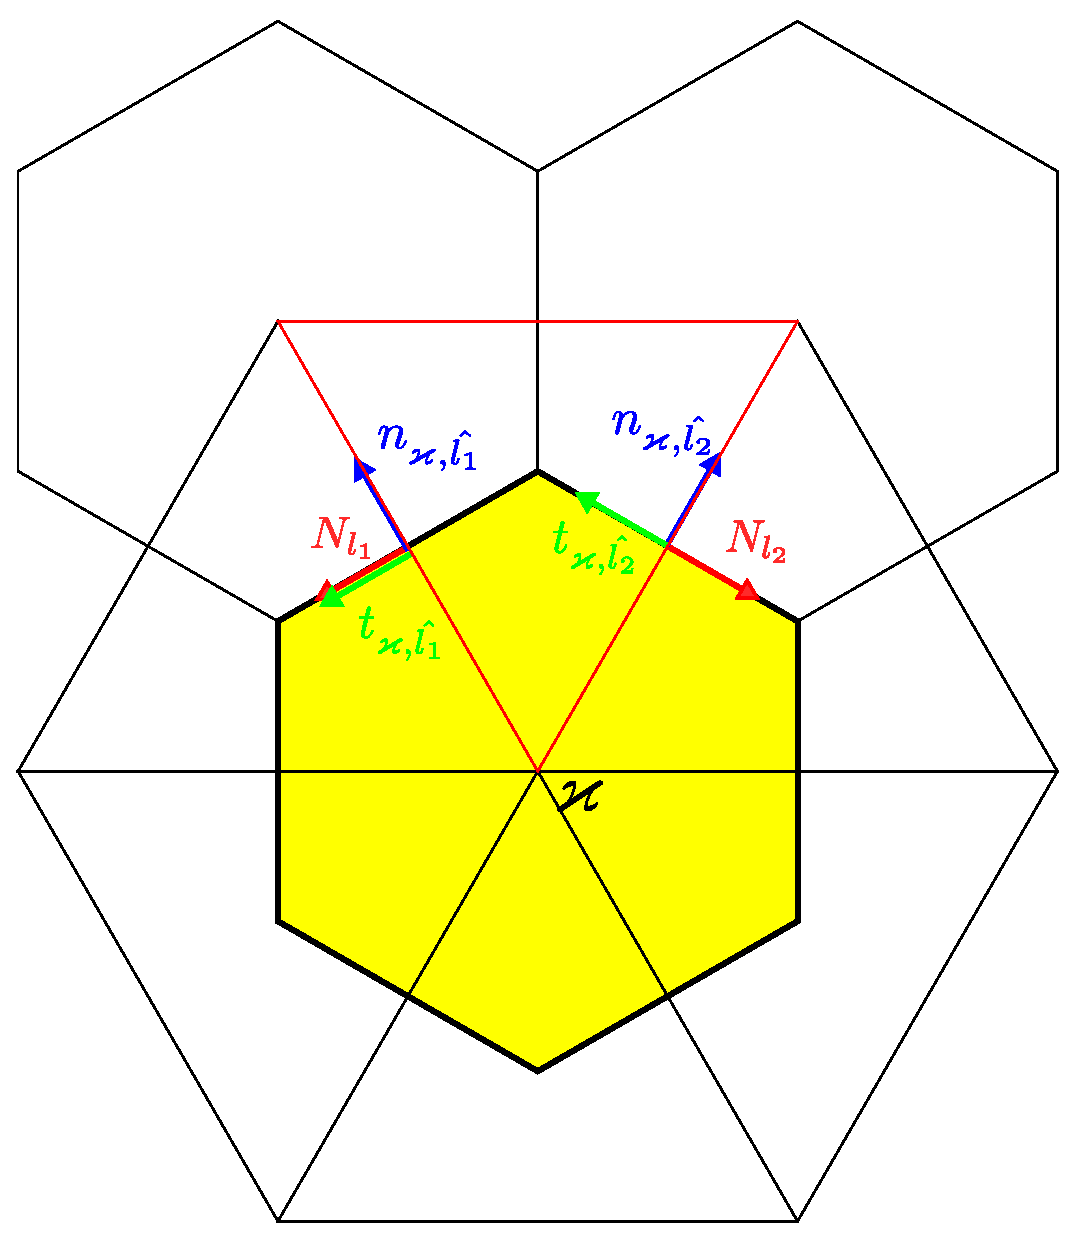
\includegraphics[width=0.7\textwidth]{dual_sign.eps}
  \end{figure}

Here, $\bm{N}_{l_1}$ and $\bm{N}_{l_2}$ are of such directions because we define the flux on downward triangle (the red one) to be outward.
On the yellow dual cell denoted by vertex $\varkappa$, the ourward unit vectors are $\bm{n}_{\varkappa, \hat{l_1}}$ and $\bm{n}_{\varkappa, \hat{l_2}}$.
Since we need $\bm{n}_{\varkappa, \hat{l}} \times \bm{t}_{\varkappa, \hat{l}}=\bm{k}_l$, where $\bm{k}_l$ denotes the unit vector in the upward direction of the local coordinate at the midpoint of edge $l$, the green $\bm{t}_{\varkappa, \hat{l_1}}$ and $\bm{t}_{\varkappa, \hat{l_2}}$ are as shown in the figure.

The curl operator is
\[\text{curl}(\bm{v})_{\varkappa} = \frac{1}{A_\varkappa}\sum\limits_{\hat{l}}v_{n_l}(\bm{N_l}\cdot\bm{t}_{\varkappa, \hat{l}})\hat{l}\]
Note the part $\bm{N_l}\cdot\bm{t}_{\varkappa, \hat{l}}$, we see that this sign is different on edges $\hat{l}$ for a dual cell $\varkappa$ ($1$ for $\hat{l_1}$ and $-1$ for $\hat{l_2}$). Therefore the previous approach we used for a divergence operator, which is to assume a uniform sign on all edges of a cell, cannot be applied here. A separate formula based on the color of an edge is not valid either, because for $\hat{l_1}$ and the bottom-right dual edge, they are of different signs.


There are some solutions to this problem, but I cannot see a simple one without modifying the GridTools. For example:
\begin{itemize}
  \item a field on both vertexes and edges
  \item a different \texttt{on\_edges()} traversal for a vertex. For example, \texttt{on\_odd\_edges()} and \texttt{on\_even\_edges()}.
\end{itemize}

 It remains to be seen whether the second proposal would be general enough. I still need to read the literature to find more operators. I think for a Laplacian there will be no such problem of multiple values on one place, or nonuniform formula on fields. But I need to find out if there are more operators involving traversing surrounding edges and treating each of them differently. Well I have to read the papers now because I am stuck here anyway :P

\end{document}
